% ----------------------------------------------------------
% Subseção Teorema central do limite
% ----------------------------------------------------------
\subsection{Teorema central do limite}
Fundamentado nos axiomas observados na Figura \ref{fig:primordial_logic_representation}, tem-se o seguinte teorema: Se a parte de subintervalos são subpartes de todo o intervalo, então essas subpartes somadas são a parte de todo o intervalo.

Assim, na Figura \ref{fig:second_logical_moment}, a negação do primeiro momento lógico nega \underline{SER}, já as subnegações dos demais momentos lógicos são subpartes que subnegam o \underline{SER}, assim essas subpartes somente negam o \underline{SER} quando somadas ou unificadas conforme o primeiro momento lógico.
	\begin{figure}[H]
	\caption{Momentos lógicos subdivididos}
	\label{fig:second_logical_moment}
	\centering
	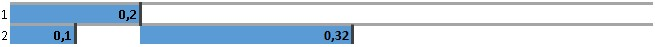
\includegraphics[scale=.85]{sections/images/second_logical_moment.jpg}
	\floatfoot{Exemplo dos dois primeiros momentos de uma expansão.}%\footnotemark}
	\end{figure}
	%\footnotetext{Fonte: note}

Na Figura \ref{fig:logical_units} pode ser observada a representação do primeiro e segundo momentos lógicos, da Figura \ref{fig:second_logical_moment}, como unidades lógicas.
	\begin{figure}[H]
	\caption{Momentos lógicos unificados}
	\label{fig:logical_units}
	\centering
	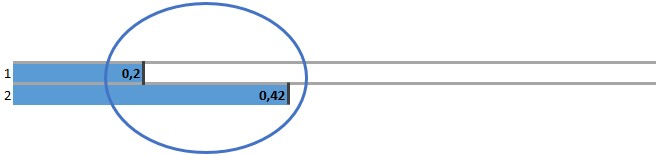
\includegraphics[scale=.85]{sections/images/logical_units.jpg}
	\floatfoot{Exemplo dos dois primeiros momentos unificados de uma expansão.}%\footnotemark}
	\end{figure}
	%\footnotetext{Fonte: note}

A dinâmica do teorema descrito acima e dos seus axiomas essenciais da lógica são observáveis cognitivamente pela construção matemática dos números naturais, reajustando a escala dos símbolos que representam cada momento lógico conforme a necessidade da expansão lógica. A matemática suporta a operação de soma, necessária na representação do teorema acima, com a aritmética de Presburguer, que é consistente, completa e decidível \cite{wiki_AritmeticaPresburger}.

O teorema e os axiomas essenciais da lógica também podem ser observáveis cognitivamente pela construção matemática dos números reais positivos (representado sem operações, como frações, raízes etc., ou seja, os decimais finitos), o qual é suportado pela teoria matemática de corpo ordenado - um subconjunto dos números reais maiores ou igual a zero e fechados para as operações de soma e produto, não sendo necessária a operação de produto e suas propriedades para a dinâmica do teorema e dos seus axiomas essenciais da lógica \cite{wiki_CorpoOrdenado}. A teoria matemática de corpo ordenado é uma teoria de primeira ordem matemática, com todos os seus axiomas descritos pela lógica de primeira ordem, tornando-a completa e decidível \cite{wiki_RealClosedField}. 

É importante observar que a lógica em sua essência não está sujeita à matemática, mas toda a matemática está restrita à lógica e, portanto, algumas de suas construções mais simples podem se aproximar mais da lógica essencial do que outras.

A unidade presente na negação (primeiro momento lógico) e nas subnegações lógicas (demais momentos lógicos) é a característica que corresponde ao eixo central do teorema central do limite. Esse teorema afirma que a distribuição amostral de uma população se aproxima de uma distribuição normal à medida que as quantidades das amostras aumentam, independente da forma da distribuição da população. Esse fato é especialmente verdadeiro para a quantidade de amostras acima de 30. Um simples teste que demonstra esse fato é o lançamento de dados não viciados. Quanto maior for o número de lançamento do dado, maior a probabilidade de o gráfico parecer com o gráfico da distribuição normal \cite{statisticshowto_teorema_central_limite}. O Apêndice \ref{app:algoritmos} explica o algoritmo Distribution\_PROB com o intuito que clarificar a essência probabilística do teorema central do limite.

A Figura \ref{fig:statisticsbyjim_central_limit_theorem} ilustra o teorema central do limite quanto ao fato probabilístico da aproximação do histograma à distribuição normal e da aproximação das colunas ou faixas desse gráfico à mediana a medida que as amostras aumentam. No gráfico são distribuídas 500.000 amostras randomicamente e divididas em colunas com range amostral ou intervalos de ([5-vermelho], [20-azul] e [40-verde]), a cor cinza mostra os valores distorcidos da população \cite{statisticsbyjim_central_limite_theorem_explainded}.
	\begin{figure}[H]
	\caption{Aproximação do histograma à distribuição normal e da aproximação das colunas desse gráfico à mediana}
	\label{fig:statisticsbyjim_central_limit_theorem}
	\centering
	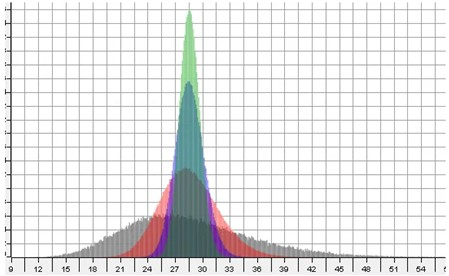
\includegraphics[scale=1.2]{sections/images/statisticsbyjim_central_limit_theorem.jpg}
	\floatfoot{500.000 amostras distribuídas randomicamente em cada range amostral de ([5-vermelho], [20-azul] e [40-verde] \cite{statisticsbyjim_central_limite_theorem_explainded}. \protect\footnotemark}
	\end{figure}
	\footnotetext{\url{www.statisticsbyjim.com/basics/central-limit-theorem}}

É importante notar, conforme Figura \ref{fig:trend_chart_of_normal_distribution}, que o equilíbrio ou sincronismo probabilístico à direita e esquerda da mediana, causadas pela distribuição dos momentos lógicos unificados, podem ilustrar a doutrina dos contrários de Heráclito de Éfeso \cite{brasilescola_heraclito}.
	\begin{figure}[H]
	\caption{Sincronismo  probabilístico das amostras contrárias em relação à mediana}
	\label{fig:trend_chart_of_normal_distribution}
	\centering
	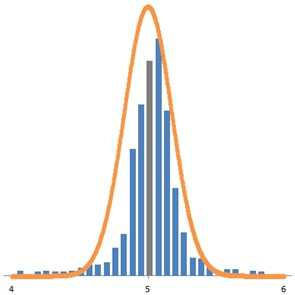
\includegraphics[scale=1.1]{sections/images/trend_chart_of_normal_distribution.jpg}
	\floatfoot{Exemplo de uma distribuição que se aproxima da distribuição normal.}%\footnotemark}
	\end{figure}
	%\footnotetext{Fonte: note}

Na Tabela \ref{tab:10000_all} está a probabilidade da distribuição binomial entre 100 a 10000 amostras, consonante às amostras unificadas, Figura \ref{fig:logical_units}, ou médias amostrais tratadas no teorema central do limite.

A distribuição binomial se comporta como o lançamento de moedas (cara ou coroa), no caso da primeira linha da tabela, distribuição de 100 amostras, tem-se 101 possibilidades, de 0 a 100, como se fossem lançadas 100 moedas somando suas faces voltadas para cima, podendo ser 0 para as caras e 1 para as coroas, por exemplo. Assim, se as 100 moedas lançadas saírem como cara a soma será igual 0 e se todas elas saírem como coroa a soma será 100. Essa soma é uma combinação de possibilidades não uma permutação, ou seja, na permutação [0, 1] é uma possibilidade diferente de [1, 0], na combinação essa é uma possiblidade, porém com duas probabilidades de ocorrência. Logo, a somatória correspondente a 100\% de cara ou 100\% de coroa correspondem a 1 possibilidade cada uma, já as demais somatórias têm maior possibilidade de ocorrer. Para essa primeira linha da tabela, 100 moedas, 99,994\% de todas as possibilidades somam entre 31 a 70. 

A construção dessa tabela se deu com a fórmula da probabilidade binomial geral, que representa uma distribuição uniforme, por meio do algoritmo BinomialDistribuion\_PROB clarificado no Apêndice \ref{app:algoritmos} \cite{mathisfun_binomial_distribution}.
	\begin{align*}
	f(k;n,p) &= \binom{n}{k} p^k(1 - p)^{n-k}
	\end{align*}
Foi utilizada a distribuição binomial nesta seção do estudo, mas poderia ser utilizada outras distribuições discretas, como o lançamento de dados não viciados, e as observações deste estudo continuariam as mesmas, pois o teorema central do limite é independente da forma da distribuição da população \cite{statisticsbyjim_central_limite_theorem_explainded}.
\begin{table}[H]
\caption{Probabilidade da distribuição binomial}
\floatfoot{Tabela gerada pelo algoritmo BinomialDistribuion\_PROB com a distribuição binomial de 100 a 10000. \footnotemark}
\label{tab:10000_all}
\resizebox{\textwidth}{!}{%
\begin{tabular}{cccc
>{\columncolor[HTML]{8D3CE1}}c 
>{\columncolor[HTML]{5754D6}}c 
>{\columncolor[HTML]{8FFFFB}}c c}
\hline
\cellcolor[HTML]{95ABEC} & \cellcolor[HTML]{95ABEC} & \multicolumn{2}{c}{\cellcolor[HTML]{95ABEC}} & \cellcolor[HTML]{95ABEC} & \cellcolor[HTML]{95ABEC} & \cellcolor[HTML]{95ABEC} & \cellcolor[HTML]{95ABEC} \\
\cellcolor[HTML]{95ABEC} & \cellcolor[HTML]{95ABEC} & \multicolumn{2}{c}{\cellcolor[HTML]{95ABEC}} & \cellcolor[HTML]{95ABEC} & \cellcolor[HTML]{95ABEC} & \cellcolor[HTML]{95ABEC} & \cellcolor[HTML]{95ABEC} \\
\multirow{-3}{*}{\cellcolor[HTML]{95ABEC}\textbf{Meta}} & \multirow{-3}{*}{\cellcolor[HTML]{95ABEC}\textbf{\begin{tabular}[c]{@{}c@{}}Soma do \\ Range\end{tabular}}} & \multicolumn{2}{c}{\multirow{-3}{*}{\cellcolor[HTML]{95ABEC}\textbf{Range}}} & \multirow{-3}{*}{\cellcolor[HTML]{95ABEC}\textbf{\begin{tabular}[c]{@{}c@{}}Total de \\ Amostras\end{tabular}}} & \multirow{-3}{*}{\cellcolor[HTML]{95ABEC}\textbf{\begin{tabular}[c]{@{}c@{}}Amostras \\ do Range\end{tabular}}} & \multirow{-3}{*}{\cellcolor[HTML]{95ABEC}\textbf{\begin{tabular}[c]{@{}c@{}}\% das \\ Amostras \\ do Range\end{tabular}}} & \multirow{-3}{*}{\cellcolor[HTML]{95ABEC}\textbf{\begin{tabular}[c]{@{}c@{}}Range de $\approx$ 28\% \\ das Amostras \\ do Range\end{tabular}}} \\ \hline
99,99\% & 99,994\% & 31 & 70 & \textbf{101} & \textbf{39} & \textbf{38\%} & 72,87\% \\ \hline
\cellcolor[HTML]{C0C0C0}99,99\% & \cellcolor[HTML]{C0C0C0}99,992\% & \cellcolor[HTML]{C0C0C0}73 & \cellcolor[HTML]{C0C0C0}128 & \textbf{201} & \textbf{55} & \textbf{27\%} & \cellcolor[HTML]{C0C0C0}{\color[HTML]{000000} 71,11\%} \\ \hline
99,99\% & 99,991\% & 117 & 184 & \textbf{301} & \textbf{67} & \textbf{22\%} & 72,73\% \\ \hline
\cellcolor[HTML]{C0C0C0}99,99\% & \cellcolor[HTML]{C0C0C0}99,990\% & \cellcolor[HTML]{C0C0C0}162 & \cellcolor[HTML]{C0C0C0}239 & \textbf{401} & \textbf{77} & \textbf{19\%} & \cellcolor[HTML]{C0C0C0}70,62\% \\ \hline
99,99\% & 99,991\% & 207 & 294 & \textbf{501} & \textbf{87} & \textbf{17\%} & 73,64\% \\ \hline
\cellcolor[HTML]{C0C0C0}99,99\% & \cellcolor[HTML]{C0C0C0}99,991\% & \cellcolor[HTML]{C0C0C0}253 & \cellcolor[HTML]{C0C0C0}348 & \textbf{601} & \textbf{95} & \textbf{15\%} & \cellcolor[HTML]{C0C0C0}72,96\% \\ \hline
99,99\% & 99,991\% & 299 & 402 & \textbf{701} & \textbf{103} & \textbf{14\%} & 72,69\% \\ \hline
\cellcolor[HTML]{C0C0C0}99,99\% & \cellcolor[HTML]{C0C0C0}99,990\% & \cellcolor[HTML]{C0C0C0}346 & \cellcolor[HTML]{C0C0C0}455 & \textbf{801} & \textbf{109} & \textbf{13\%} & \cellcolor[HTML]{C0C0C0}72,69\% \\ \hline
99,99\% & 99,991\% & 392 & 509 & \textbf{901} & \textbf{117} & \textbf{12\%} & 72,86\% \\ \hline
\cellcolor[HTML]{C0C0C0}99,99\% & \cellcolor[HTML]{C0C0C0}99,991\% & \cellcolor[HTML]{C0C0C0}439 & \cellcolor[HTML]{C0C0C0}562 & \textbf{1001} & \textbf{123} & \textbf{12\%} & \cellcolor[HTML]{C0C0C0}73,16\% \\ \hline
99,99\% & 99,991\% & 486 & 615 & \textbf{1101} & \textbf{129} & \textbf{11\%} & 73,54\% \\ \hline
\cellcolor[HTML]{C0C0C0}99,99\% & \cellcolor[HTML]{C0C0C0}99,991\% & \cellcolor[HTML]{C0C0C0}533 & \cellcolor[HTML]{C0C0C0}668 & \textbf{1201} & \textbf{135} & \textbf{11\%} & \cellcolor[HTML]{C0C0C0}71,45\% \\ \hline
99,99\% & 99,991\% & 580 & 721 & \textbf{1301} & \textbf{141} & \textbf{10\%} & 72,06\% \\ \hline
\cellcolor[HTML]{C0C0C0}99,99\% & \cellcolor[HTML]{C0C0C0}99,990\% & \cellcolor[HTML]{C0C0C0}628 & \cellcolor[HTML]{C0C0C0}773 & \textbf{1401} & \textbf{145} & \textbf{10\%} & \cellcolor[HTML]{C0C0C0}72,68\% \\ \hline
99,99\% & 99,991\% & 675 & 826 & \textbf{1501} & \textbf{151} & \textbf{10\%} & 73,31\% \\ \hline
\cellcolor[HTML]{C0C0C0}99,99\% & \cellcolor[HTML]{C0C0C0}99,990\% & \cellcolor[HTML]{C0C0C0}723 & \cellcolor[HTML]{C0C0C0}878 & \textbf{1601} & \textbf{155} & \textbf{9\%} & \cellcolor[HTML]{C0C0C0}71,76\% \\ \hline
99,99\% & 99,991\% & 770 & 931 & \textbf{1701} & \textbf{161} & \textbf{9\%} & 72,49\% \\ \hline
\cellcolor[HTML]{C0C0C0}99,99\% & \cellcolor[HTML]{C0C0C0}99,990\% & \cellcolor[HTML]{C0C0C0}818 & \cellcolor[HTML]{C0C0C0}983 & \textbf{1801} & \textbf{165} & \textbf{9\%} & \cellcolor[HTML]{C0C0C0}73,20\% \\ \hline
99,99\% & 99,990\% & 866 & 1035 & \textbf{1901} & \textbf{169} & \textbf{8\%} & 71,90\% \\ \hline
\cellcolor[HTML]{C0C0C0}99,99\% & \cellcolor[HTML]{C0C0C0}99,990\% & \cellcolor[HTML]{C0C0C0}914 & \cellcolor[HTML]{C0C0C0}1087 & \textbf{2001} & \textbf{173} & \textbf{8\%} & \cellcolor[HTML]{C0C0C0}72,67\% \\ \hline
99,99\% & 99,990\% & 1394 & 1607 & \textbf{3001} & \textbf{213} & \textbf{7\%} & 71,86\% \\ \hline
\cellcolor[HTML]{C0C0C0}99,99\% & \cellcolor[HTML]{C0C0C0}99,991\% & \cellcolor[HTML]{C0C0C0}1877 & \cellcolor[HTML]{C0C0C0}2124 & \textbf{4001} & \textbf{247} & \textbf{6\%} & \cellcolor[HTML]{C0C0C0}72,47\% \\ \hline
99,99\% & 99,990\% & 2363 & 2638 & \textbf{5001} & \textbf{275} & \textbf{5\%} & 72,38\% \\ \hline
\cellcolor[HTML]{C0C0C0}99,99\% & \cellcolor[HTML]{C0C0C0}99,990\% & \cellcolor[HTML]{C0C0C0}2850 & \cellcolor[HTML]{C0C0C0}3151 & \textbf{6001} & \textbf{301} & \textbf{5\%} & \cellcolor[HTML]{C0C0C0}72,75\% \\ \hline
99,99\% & 99,990\% & 3338 & 3663 & \textbf{7001} & \textbf{325} & \textbf{4\%} & 72,32\% \\ \hline
\cellcolor[HTML]{C0C0C0}99,99\% & \cellcolor[HTML]{C0C0C0}99,990\% & \cellcolor[HTML]{C0C0C0}3827 & \cellcolor[HTML]{C0C0C0}4174 & \textbf{8001} & \textbf{347} & \textbf{4\%} & \cellcolor[HTML]{C0C0C0}72,18\% \\ \hline
99,99\% & 99,990\% & 4316 & 4685 & \textbf{9001} & \textbf{369} & \textbf{4\%} & 72,23\% \\ \hline
\cellcolor[HTML]{C0C0C0}99,99\% & \cellcolor[HTML]{C0C0C0}99,990\% & \cellcolor[HTML]{C0C0C0}4806 & \cellcolor[HTML]{C0C0C0}5195 & \textbf{10001} & \textbf{389} & \textbf{3\%} & \cellcolor[HTML]{C0C0C0}72,42\% \\ \hline
\end{tabular}%
}
\end{table}
\footnotetext{O Apêndice \ref{app:algorithms} é dedicado a clarificar o algoritmo BinomialDistribuion\_PROB e validar o fórmula da probabilidade binomial geral usada por ele.}
\vspace{-8mm}
\begin{description}
   \item[Meta] Porcentagem das amostras observadas;
   \item[Soma do Range] Porcentagem que o \textbf{"Range"} atingiu a \textbf{"Meta"}, da mediana para as bordas, descentralizado;
   \item[Range] Range de amostras onde a \textbf{"Meta"} foi atingida do \textbf{"Total de Amostras"};
   \item[Total de Amostras] Exibe o range total avaliado, no caso da primeira linha da tabela o valor 101 corresponde às possibilidades de 0 a 100;
   \item[Amostras do Range] Quantidade de amostras do \textbf{"Range"};
   \item[Porcentagem das Amostras do Range] Porcentagem que o \textbf{"Range} representa do \textbf{"Total de Amostras"};
   \item[Range de $\approx$ 28\% das Amostras do Range] Esse range é  subconjunto do \textbf{"Range"}, formado a partir da mediana somando 14\% a direita e a esquerda, totalizando 28\%. Esses 28\% correspondem a aproximadamente 72\% das \textbf{"Amostras do Range"} e está por sua vez correspondem a 99,99\% da população total. O restante, que representam 72\% do tamanho do \textbf{"Range"}, correspondem a aproximadamente 28\% das amostras. Isso condiz com o Princípio de Pareto também conhecido como a regra do 80/20 e que também pode ser 70/30 ou 90/10, por exemplo \cite{wiki_pareto_principle}.
\end{description}
\bigbreak


Pode-se observar que a medida que as amostras aumentam, a porcentagem ocupada por 99,99\% das amostras \textbf{"\% das Amostras do Range"} tende a diminuir ainda que cada vez mais devagar, por mais que a quantidade de amostras que representam essa porcentagem tenda a aumentar \textbf{"Amostras do Range"}.

A coluna de \textbf{"Amostras do Range"}, da Tabela \ref{tab:10000_all}, setas azuis no gráfico da Figura \ref{fig:total_comparison_chart_with_99_range} estarão cada vez mais próximas do centro do gráfico, proporcionalmente, ou seja, apesar de aumentar a quantidade de \textbf{"Amostras do Range"}, a proporção que elas assumem no \textbf{"Total de Amostras"}  diminuem. As setas em roxo do gráfico representam a coluna \textbf{"Total de Amostras"} da Tabela \ref{tab:10000_all}. 
	\begin{figure}[H]
	\caption{Comparação do total de amostras com o range de 99,99\% }
	\label{fig:total_comparison_chart_with_99_range}
	\centering
	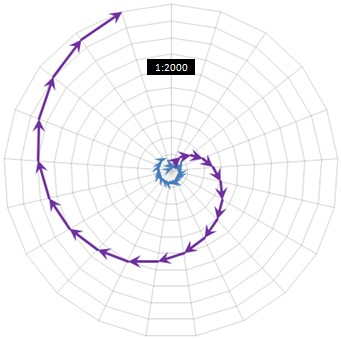
\includegraphics[scale=.9]{sections/images/total_comparison_chart_with_99_range.jpg}
	\floatfoot{As setas em roxo representam a coluna "Total das Amostras" e as em azul a coluna "Amostras do Range" da Tabela \ref{tab:10000_all}. \footnotemark}
	\end{figure}
	\footnotetext{O gráfico da Figura \ref{fig:total_comparison_chart_with_99_range} representa as 20 primeiras linhas da Tabela \ref{tab:10000_all}, pois sofrem incrementos iguais, de 100 amostras, em cada linha. A linha 21 em diante sofrem incremento de 1000 amostras a cada linha.}

No endereço \url{https://www.mathsisfun.com/data/quincunx.html} existe uma ferramenta chamada Quincunx ou Galton Board que exemplifica dinamicamente o que as figuras acima mostram. Uma explicação sobre o funcionamento dessa ferramenta pode ser vista em \url{https://www.mathsisfun.com/data/quincunx-explained.html}. 